\chapter{Test Cases}
\label{ch:testcases}
The Test Cases presented in this study serve the purpose of comparing and validating different drill string models. All the parameters and results from AS model and ExxonMobil model are provided, therefore; other models can use these Test Cases for validation. All the suggested Test Cases are off-bottom scenarios since AS model only has torsional modeling capability. However, these Test Cases can provide reliable means of cross-checking and comparing the performances of various models. 

Total six Test Cases are presented. Specifically, Test Cases 1 and 3 encompass scenarios involving vertical wells, with the distinction in the presence BHA components.Similarly, Test Cases 2 and 4 are the deviated well scenarios with 60\textdegree inclination angle. The only difference between Test Case 2 and 4 are the exitance of BHA components. In addition, to analyze the effect of frictional factors, Test Cases 2 and 4 are further divided into Test Case 2a, 2b, Test Case 4a, and 4b. This extension of Test Cases was established for deviated wells, as vertical wells experience no friction where the drill string - well bore friction is assumed to be only Coulomb friction from the normal force at drill string. \tablename~\ref{Test_case_summary} summarizes the scenarios for each Test Case. 


\begin{table}[!hbt]
    \centering
    \begin{tabular}{|c|c|c|c|c|c|c|}
        \hline
        \textbf{Test Cases} & \textbf{Well Type} & \textbf{Static FF} & \textbf{Dynamic FF}& \textbf{BHA}\\
        \hline
        Test Case 1 & Vertical & 0 & 0 & X\\
        \hline
        Test Case 2a & Deviated (60\textdegree{}) & 0.5 & 0.5 & X \\
        \hline
        Test Case 2b & Deviated (60\textdegree{}) & 0.5 & 0.25 & X \\
        \hline
        Test Case 3 & Vertical & 0 & 0 & O\\                                                
        \hline
        Test Case 4a & Deviated (60\textdegree{}) & 0.5 & 0.5 & O \\                                                  
        \hline
        Test Case 4b & Deviated (60\textdegree{}) & 0.5 & 0.25 & O \\                                                     
        \hline
    \end{tabular}
    \caption[Scenarios of different Test Cases]{Scenarios of different Test Cases.}
    \label{Test_case_summary}
\end{table} 
Additionally, the viscous damping is neglected for the simplicity of the test in this project, but it can be included in the future sutdy. Also, The test was conducted by assuming the top drive velocity to be increased from 0 RPM to 40 RPM at 1 second and maintained the velocity for rest of the time. The top drive velocity is shown in \figurename~\ref{figure_topdrive_VSP}

\begin{figure}[!hbt]
  \centering
  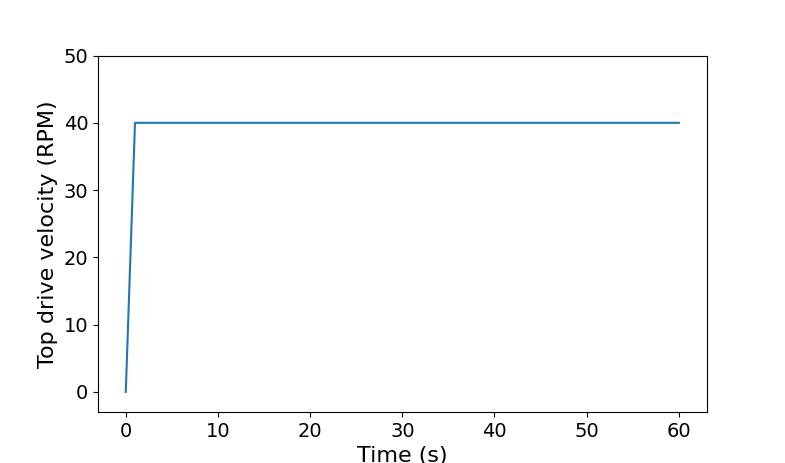
\includegraphics[width=3.5in]{TopdriveVSP}
  \caption[Top drive set velocity]{Top drive set velocity}\label{figure_topdrive_VSP}
\end{figure}

Some of the findings and modifications made on the provided source code of the AS and ExxonMobil models are presented in this chapter. In the AS model, the effect of the PI controller was tested. Also, some of the issues with the Python ver. of AS model are shown. Since this issue has not been resolved yet, the Python ver. was only executed with Test Case 1. On the other hand, The problem with the ExxonMobil model's on-bottom case has been resolved. In addition, there is an issue with mud motor that we are addressing. 
\section{Terminology}
\subsection{With BHA vs without BHA}

The Test Cases enables comparing drilling scenarios with and without the BHA components. 
%It introduces specific parameters that differ from the rest of the drill pipe in terms of weight and diameter. However, when the BHA is not present, that particular section of the drill pipe above the bit will have the same weight and diameter as the rest of the drill pipe.

\textbf{Without BHA}: To maintain simplicity and establish a baseline, we begin the study with a single drill pipe configuration. This configuration represents the most straightforward drilling arrangement, with a solitary pipe running from the surface to the drill bit. In this case, the weight and diameter of the entire drill pipe, including the section above the bit, are uniform.

\textbf{With BHA}: Introduce the BHA into the system and examine its impact on drilling dynamics. The BHA's distinct parameters, such as its weight and diameter, will be considered in the analysis to understand how it influences drilling performance. By conducting these comparative analyses, we aim to gain valuable insights into the effects of the BHA on the drill string's behavior and the overall drilling process.
%In the next subsection we will explore additional configurations with varying BHA designs and properties to further investigate their influence on drilling efficiency and performance. These test cases will enable us to optimize drilling operations and develop a comprehensive understanding of how the presence or absence of the BHA affects the system's behavior.

\subsection{Same vs different FF}

Most of the drill string models including A-S and ExxonMobil model take in to account both static and dynamic friction factors (FF). The friction factors will affect the drill string vibration in deviated well, since the interaction between the drill string and the wellbore wall becomes complex due to the influence of gravity and the inclination angle.
%but the disparity in FF values is expected to be more pronounced in inclined wells compared to vertical ones. 
Therefore, to gain insights into the impact of FF values on drilling dynamics, a detailed investigation is warranted.
%This results in differing frictional forces acting on the drill string as it traverses the wellbore. As a consequence, the FF values play a crucial role in affecting the drilling performance and behavior.

\textbf{Same FF}: Test conducted with same value of static and dynamic friction. This simulates the model with no effect of dynamic friction. 

\textbf{Different BHA}: Test conducted with different value between static and dynamic friction. This test will help analyze the effect of dynamic friction in the system.

\section{Test Case 1 - Vertical well without BHA}
The model parameters and schematic of the wellbore surveys and drill string components are shown in  \tablename~\ref{table_verticalwell_input} and \figurename~\ref{figure_verticalwell}. The ExxonMobil model and Matlab ver.\ A-S model uses metric units while Python ver.\ A-S model uses imperial units. For the future convenience, the tables in this chapter contains both imperial and metric units.

\begin{figure}[!hbt]
  \centering
  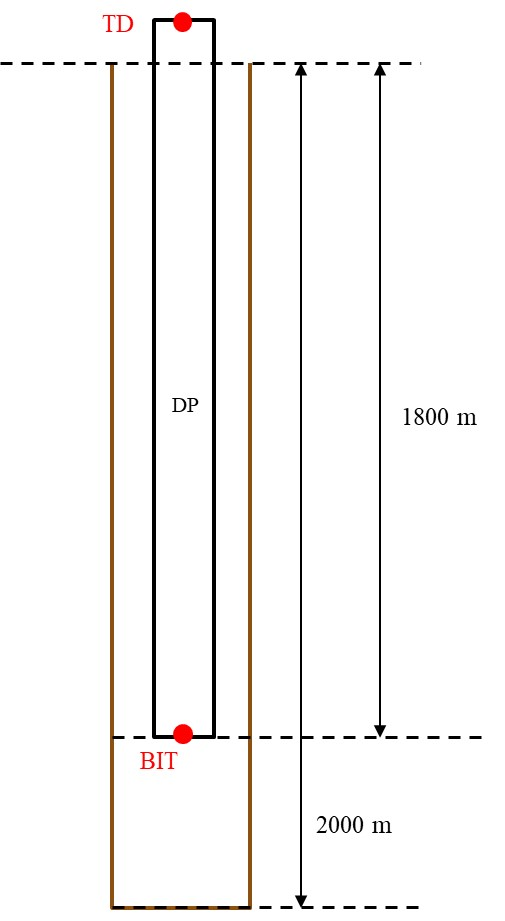
\includegraphics[width=1.5in]{VerticalWellConfig}
  \caption[Schematic of well and drill string for model comparison.]{Schematic of well and drill string for model comparison.}\label{figure_verticalwell}
\end{figure}

\begin{testcasetable}
$\rho$ & 490.6 $lb/ft^3$ & 7850 $kg/m^3$ & Drill pipe density \\                                                  
\hline
G & 1.67$\cdot$10$^{9}$ $lbf/ft^2$ & 7.99$\cdot$10$^{10}$ $Pa$  & Shear modulus \\                                                  
\hline
OD & 5.88 $in$ & 0.15 $m$ & Drill pipe outer diameter\\                                                       
\hline
ID & 5.00 $in$ & 0.127 $m$ & Drill pipe inner diameter  \\                                                      
\hline
MD & 6561 $ft$ & 2000 $m$ & Measured depth\\                                                              
\hline
TVD & 6561 $ft$ & 2000 $m$ & Total vertical depth\\
\hline
Bit depth & 5905 $ft$ & 1800 $m$ & - \\ 
\hline
\end{tabularx}
\caption[Well survey data for model comparison (vertical well)]{Well survey and drill string data for model comparison (vertical well without BHA components)}\label{table_verticalwell_input}
\end{testcasetable}

\section{Test Case 2 - Deviated well without BHA}
\subsection{Test case 2a - same FF values}
The models were tested with deviated well with simple configuration of drill string. The MD of the well is 4000 m with 60$^{\circ}$ inclination from KOP of 1500 m. The drill bit is off-bottom where located at 2500 m depth. The Schematic view of wellbore and drill string are depicted in \figurename~\ref{figure_wellconfig_inclined}. The static and dynamic friction factors were set to be the same as 0.5. The parameters for the test are summarized in \tablename~\ref{table_Inclinedwell_2a_input}.

\begin{figure}[!hbt]
  \centering
  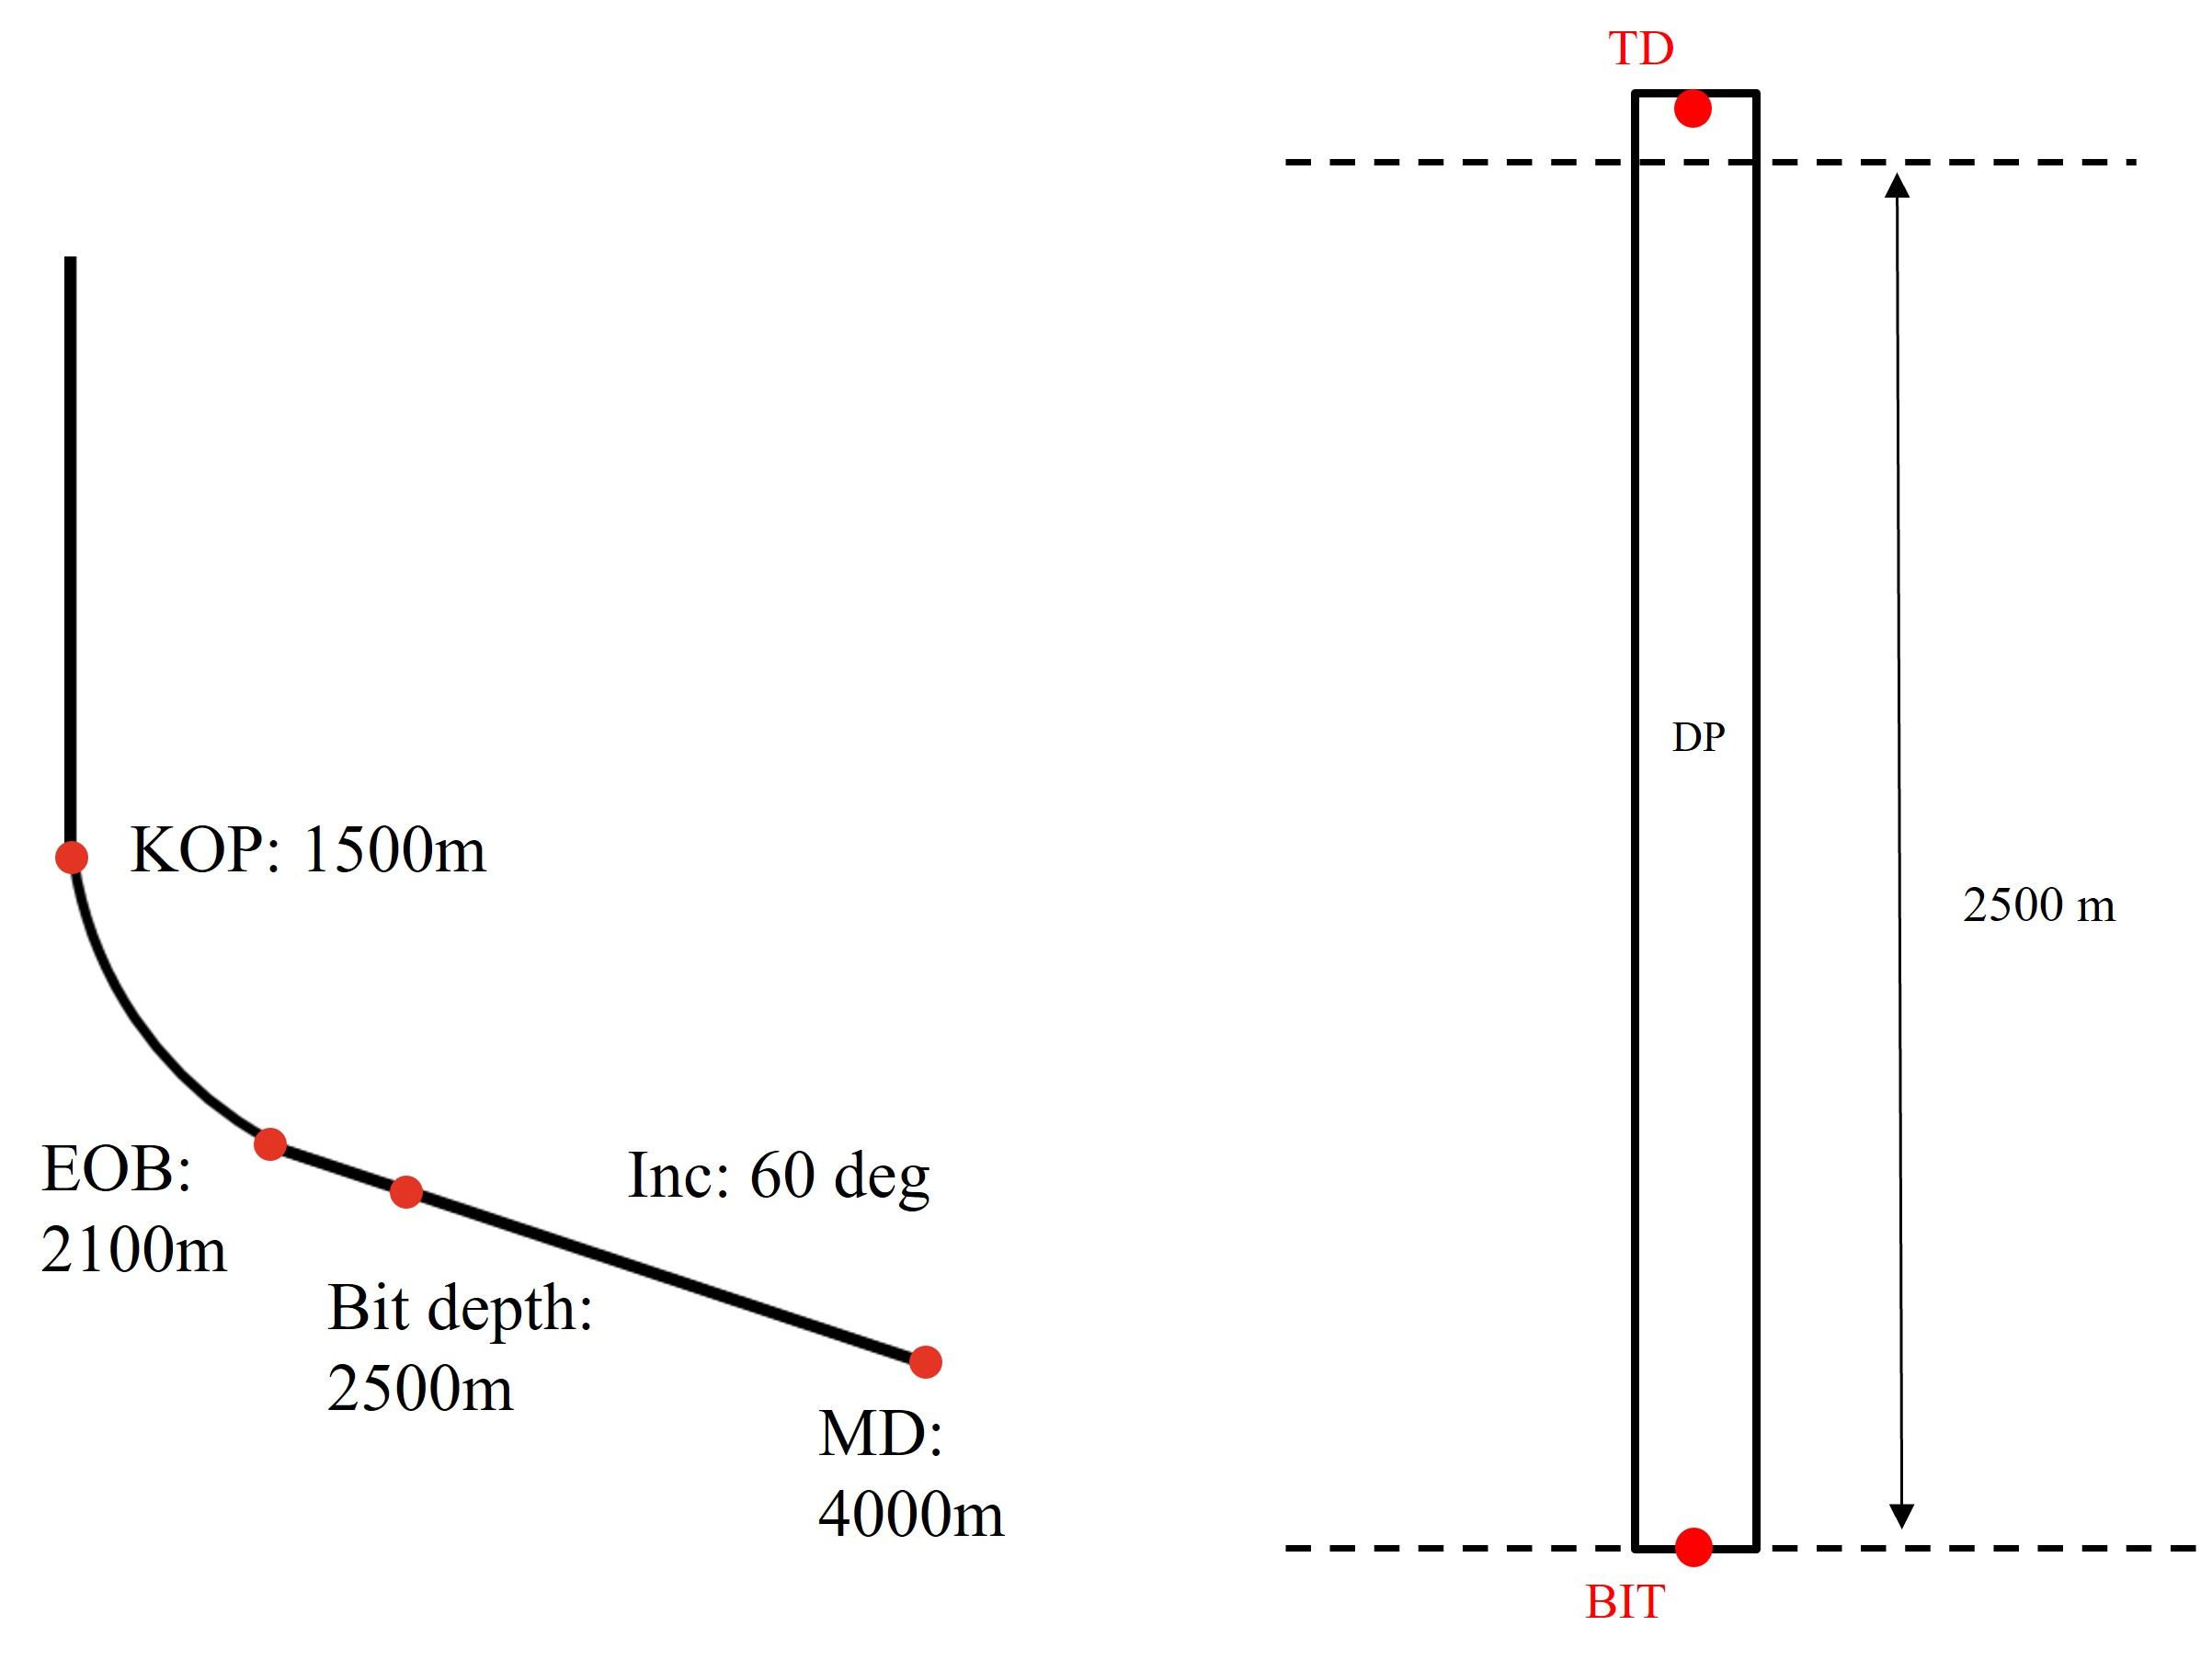
\includegraphics[width=4in]{InclinedWellConfig}
  \caption[Schematic view of Test Case 2.]{Schematic view of wellbore and drill string for Test Case 2.}\label{figure_wellconfig_inclined}
\end{figure}

\begin{testcasetable}
  $OD_{dp}$ & 5.88 $in$ & 0.15 $m$ & Drill pipe outer diameter\\                                                       
  \hline
  $ID_{dp}$ & 5.00 $in$ & 0.127 $m$ & Drill pipe inner diameter  \\                                                      
  \hline
  $\rho_{dp}$ & 490.6 $lb/ft^3$ & 7850 $kg/m^3$ & Drill pipe density \\                                                  
  \hline
  $G_{dp}$ & 1.27$\cdot$10$^{9}$ $lb/ft^2$ & 6.10$\cdot$10$^{10}$ $Pa$ & Drill pipe shear modulus\\                                                              
  \hline
  $\mu_{s}$ & 0.5 & 0.5 & Static friction factor\\
  \hline
  $\mu_{d}$ & 0.5 & 0.5 & Dynamic friction factor\\
  \hline
  $w_c$ & 10 $RPM$ & 10 $RPM$ & Cut-off angular velocity\\
  \hline
  $\theta$ & 60$^{\circ}$ & 60$^{\circ}$ & Inclination\\
  \hline
  \end{tabularx}
\caption[Input parameters for Test Case 2a]{Input parameters for Test Case 2a.}\label{table_Inclinedwell_2a_input}
\end{testcasetable}

\subsection{Test Case 2b - different FF values}
The models were tested with the exact same configuration with Test Case 2a, except different values of static and dynamic FF values. The following \tablename~\ref{table_Inclinedwell_2b_input} summarizes the input parameters. 

\begin{testcasetable}
   $OD_{dp}$ & 5.88 $in$ & 0.15 $m$ & Drill pipe outer diameter\\                                                       
   \hline
   $ID_{dp}$ & 5.00 $in$ & 0.127 $m$ & Drill pipe inner diameter  \\                                                      
   \hline
   $\rho_{dp}$ & 490.6 $lb/ft^3$ & 7850 $kg/m^3$ & Drill pipe density \\                                                  
   \hline
   $G_{dp}$ & 1.27$\cdot$10$^{9}$ $lb/ft^2$ & 6.10$\cdot$10$^{10}$ $Pa$ & Drill pipe shear modulus\\                                                              
   \hline
   $\mu_{s}$ & 0.5 & 0.5 & Static friction factor\\
   \hline
   $\mu_{d}$ & 0.25 & 0.25 & Dynamic friction factor\\
   \hline
   $w_c$ & 10 $RPM$ & 10 $RPM$ & Cut-off angular velocity\\
   \hline
   $\theta$ & 60$^{\circ}$ & 60$^{\circ}$ & Inclination\\
   \hline
\end{tabularx}
\caption[Input parameters for Test Case 2b]{Input parameters for Test Case 2b.}\label{table_Inclinedwell_2b_input}
\end{testcasetable}

\section{Test Case 3 - Vertical Well with BHA}
In this specific scenario, an additional configuration of the drill string included BHA. The BHA introduced extra components, resulting in an increase in both the weight and size of the drill string. However, the well survey data for the vertical well remained the same, except for the incorporation of the BHA. The well design, depicted in \figurename~\ref{Vert_well_conf_BHA}, remained unchanged. The specific input parameters can be found in the \tablename~\ref{Input Parameters TC3}.

\begin{figure}
  \centering
  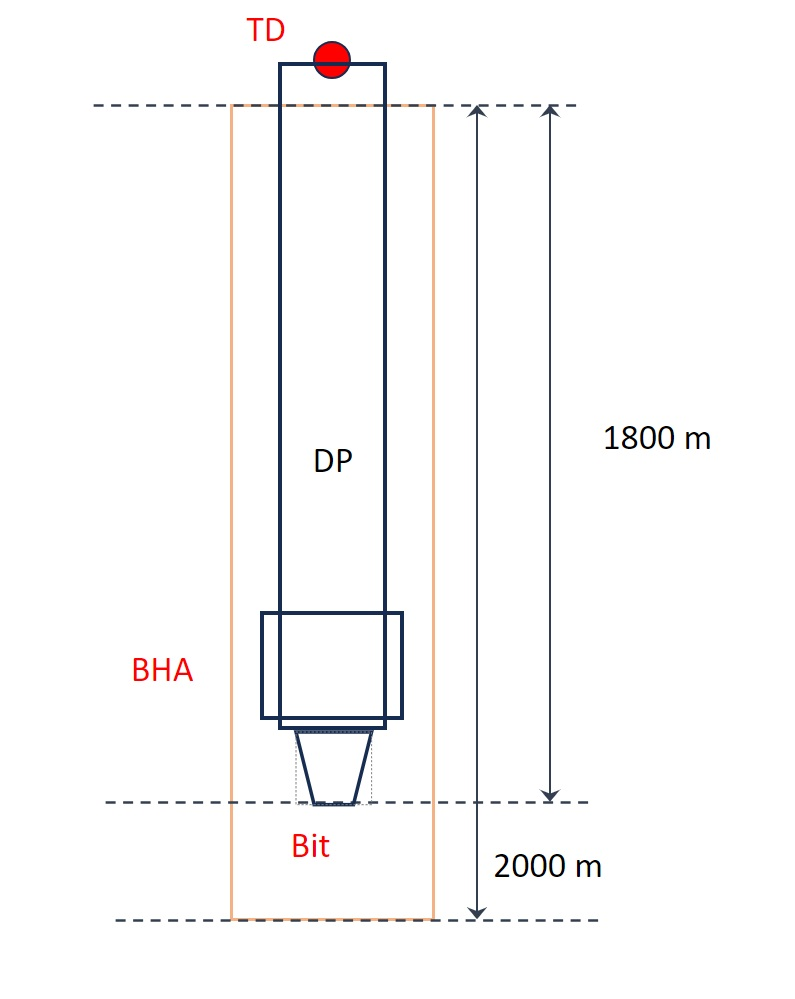
\includegraphics[width=2in]{VerticalWellConfigBHA}
  \caption{Schematic of well and drill string for model comparison}\label{Vert_well_conf_BHA}
\end{figure}


\begin{testcasetable}
    $OD_{HWDP}$ & 4.50 $in$ & 0.1143 $m$ & Heavy weight drill pipe outer diameter \\
    \hline
    $ID_{HWDP}$ & 2.50 $in$ & 0.0635 $m$ & Heavy weight drill pipe inner diameter \\
    \hline
    $OD_{DC}$ & 6.00 $in$ & 0.1524 $m$ & Drill collars outer diameter \\
    \hline
    $ID_{DC}$ & 2.00 $in$ & 0.0508 $m$ & Drill collars inner diameter \\
    \hline
    $L_{HWDP}$ & 60 $ft$ & 18.30 $m$ & Length of heavy weight drill pipe \\
    \hline
    $L_{DC}$ & 270 $ft$ & 82.30 $m$ & Length of drill collars \\
    \hline
    $\rho_{dp}$ & 490.6 $lb/ft^{3}$ & 7850 $kg/m^{3}$ & Drill pipe density \\
    \hline
    $G_{dp}$ & 1.67$\cdot$10$^{9}$ $lb/ft^2$ & 7.99$\cdot$10$^{10}$ $Pa$ & Drill pipe shear modulus\\  
    \hline
    \end{tabularx}
  \caption{Input parameters of BHA for Test Case 3}\label{Input Parameters TC3}
\end{testcasetable} 

\section{Test Case 4 - Inclined Well with BHA}
\subsection{Test Case 4a - same FF values}

The models were tested with the same input parameters from Test Case 2, with additional configuration of the drill string including BHA. Well survey data for the inclined well remained same, except for the incorporation of the BHA. The well design, depicted in \figurename~\ref{figure_wellconfig_inclined_BHA}, remained unchanged. The input parameters can be found in the  \tablename~\ref{table_Inclinedwell_4a_input}.

\begin{figure}[!hbt]
  \centering
  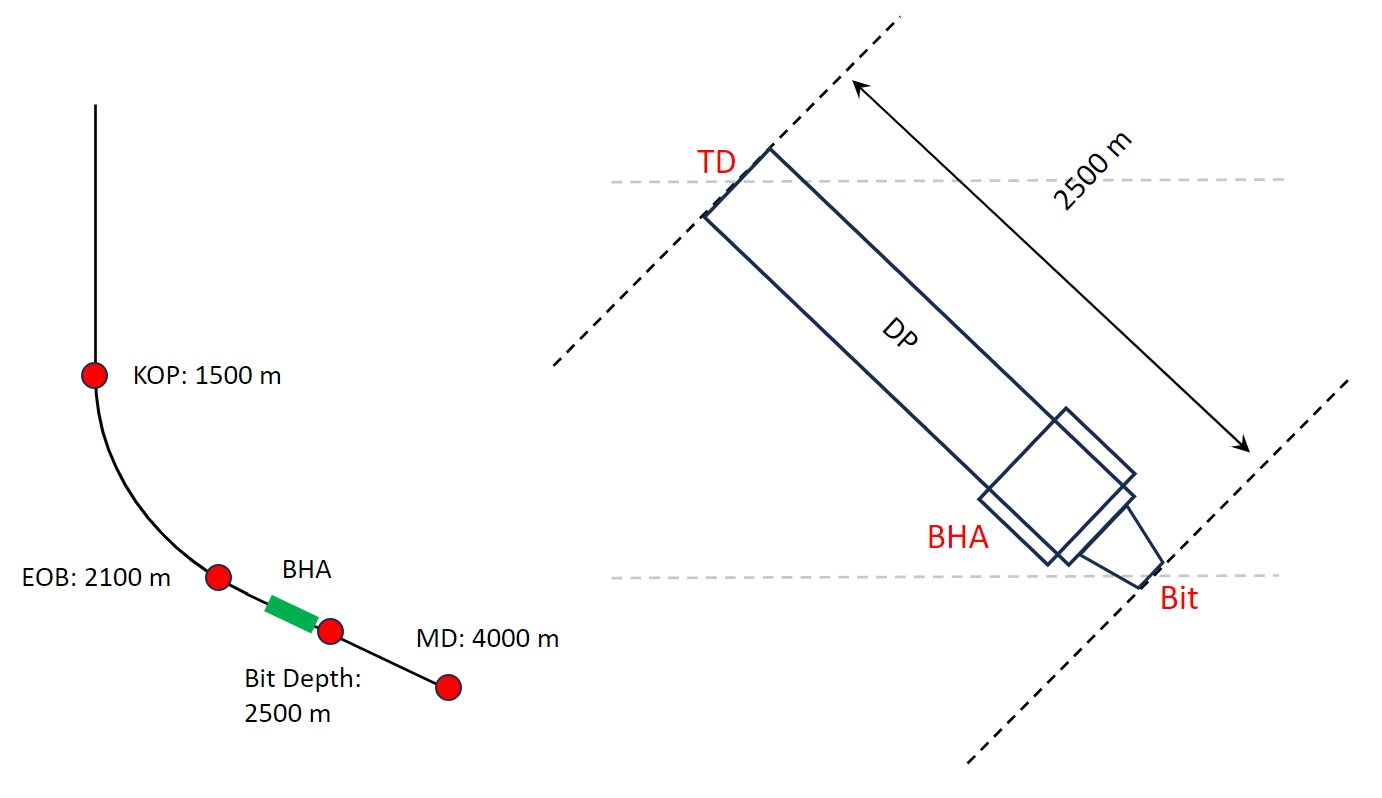
\includegraphics[width=4in]{InclinedWellConfigBHA}
  \caption[Schematic view of Test Case 4.]{Schematic view of wellbore and drill string for Test Case 4.}\label{figure_wellconfig_inclined_BHA}
\end{figure}

\begin{testcasetable}
   $OD_{HWDP}$ & 4.50 $in$ & 0.1143 $m$ & Heavy weight drill pipe outer diameter \\
   \hline
   $ID_{HWDP}$ & 2.50 $in$ & 0.0635 $m$ & Heavy weight drill pipe inner diameter \\
   \hline
   $OD_{DC}$ & 6.00 $in$ & 0.1524 $m$ & Drill collars outer diameter \\
   \hline
   $ID_{DC}$ & 2.00 $in$ & 0.0508 $m$ & Drill collars inner diameter \\                                                    
   \hline
   $L_{HWDP}$ & 60 $ft$ & 18.30 $m$ & Length of heavy weight drill pipe \\
   \hline
   $L_{DC}$ & 270 $ft$ & 82.30 $m$ & Length of drill collars \\
   \hline
   $\rho_{dp}$ & 490.6 $lb/ft^3$ & 7850 $kg/m^3$ & Drill pipe density \\                                                  
   \hline
   $G_{dp}$ & 1.27$\cdot$10$^{9}$ $lb/ft^2$ & 6.10$\cdot$10$^{10}$ $Pa$ & Drill pipe shear modulus\\  
   \hline
   $\mu_{s}$ & 0.5 & 0.5 & Static friction factor\\
   \hline
   $\mu_{d}$ & 0.5 & 0.5 & Dynamic friction factor\\
   \hline
   $w_c$ & 10 $RPM$ & 10 $RPM$ & Cut-off angular velocity\\
   \hline
   $\theta$ & 60$^{\circ}$ & 60$^{\circ}$ & Inclination\\
   \hline
   \end{tabularx}
   \caption[Input parameters for Test Case 4a]{Input parameters for Test Case 4a.}\label{table_Inclinedwell_4a_input}
\end{testcasetable}

\subsection{Test Case 4b - same FF values}

Lastly, the models were tested with the exact same configuration from the previous subsection, except with different values of static and dynamic FF values. The following \tablename~\ref{table_Inclinedwell_4b_input} summarizes the input parameters. 

\begin{testcasetable}
   $OD_{HWDP}$ & 4.50 $in$ & 0.1143 $m$ & Heavy weight drill pipe outer diameter \\
   \hline
   $ID_{HWDP}$ & 2.50 $in$ & 0.0635 $m$ & Heavy weight drill pipe inner diameter \\
   \hline
   $OD_{DC}$ & 6.00 $in$ & 0.1524 $m$ & Drill collars outer diameter \\
   \hline
   $ID_{DC}$ & 2.00 $in$ & 0.0508 $m$ & Drill collars inner diameter \\                                                    
   \hline
   $L_{HWDP}$ & 60 $ft$ & 18.30 $m$ & Length of heavy weight drill pipe \\
   \hline
   $L_{DC}$ & 270 $ft$ & 82.30 $m$ & Length of drill collars \\
   \hline
   $\rho_{dp}$ & 490.6 $lb/ft^3$ & 7850 $kg/m^3$ & Drill pipe density \\                                                  
   \hline
   $G_{dp}$ & 1.27$\cdot$10$^{9}$ $lb/ft^2$ & 6.10$\cdot$10$^{10}$ $Pa$ & Drill pipe shear modulus\\                                                                
   \hline
   $\mu_{s}$ & 0.5 & 0.5 & Static friction factor\\
   \hline
   $\mu_{d}$ & 0.25 & 0.25 & Dynamic friction factor\\
   \hline
   $w_c$ & 10 $RPM$ & 10 $RPM$ & Cut-off angular velocity\\
   \hline
   $\theta$ & 60$^{\circ}$ & 60$^{\circ}$ & Inclination\\
   \hline
   \end{tabularx}
\caption[Input parameters for Test Case 4b.]{Input parameters for Test Case 4b.}\label{table_Inclinedwell_4b_input}
\end{testcasetable}
